\chapter{What It Means to Fall Behind}

The previous chapter separated money from capital. Money becomes capital only when it has enough amount, enough time, and enough wisdom standing behind it. This chapter adds another uncomfortable condition: the world does not wait for us to become ready.

A person can be short of money and still have hope. A person can be short of knowledge and still begin learning. But a person without any sense of crisis is in a more dangerous state. Without pressure from the future, the mind easily accepts today as normal, average as sufficient, and ``almost'' as achievement.

Wealth freedom is not only the day when you no longer need to sell your time for basic living. It is also the long process of refusing to become obsolete. These two goals now stand together:

\begin{enumerate}
\item One day, you should no longer have to sell your time merely to survive.
\item One day, you should not be left behind; you should move toward the top 20\%, and perhaps the top 1\%.
\end{enumerate}

The second goal is harsher than it first appears, because most people do not know where they really stand.

\section*{Average Is a Dangerous Illusion}

In daily life, many people use a vague standard: as long as I am above average, I am not behind. The problem is that human beings are not good at locating themselves objectively.

A familiar example is driving. In many surveys, a large majority of drivers believe their skill is above average. Mathematically, this cannot be true. Yet each person has reasons: I am careful, I have experience, I know the roads, I have seen worse drivers. The feeling is persuasive from the inside.

This is often called the Lake Wobegon effect: the tendency for people to imagine themselves above average. A related pattern, the Dunning--Kruger effect, describes how people with weak ability often overestimate themselves precisely because their ability is too weak to judge ability well.

The pattern is visible everywhere. People who rarely do anything well are often quick to dismiss others: they could do it too, they simply do not care to. Meanwhile, people who are genuinely strong tend to be more cautious. They know what serious work costs. They have seen the distance between amateur appearance and professional substance. They have less need to declare themselves superior because they understand the standards.

The deeper reason is simple:

\begin{quote}
We do not perceive the whole world. We judge ourselves mainly against the small world we can see.
\end{quote}

If a person lives in a narrow pond, being above average in that pond may feel satisfying. But the pond is not the world.

This is why ``passing'' can be so misleading. In school, 60 points is often treated as enough. The extra 10 points above 50 may be seen as a buffer, a mercy, a correction for measurement. But the hidden message is severe: those after the bottom 40\% are behind. School softens this message because most students can pass something. Society is less forgiving.

After entering the real world, many people discover that ``passing'' has almost no market value. In many fields, the first 20\% capture most of the scarce resources. The Pareto pattern appears again and again: a minority receives the majority of attention, trust, income, opportunity, and capital.

So the standard changes:

\[
\text{school comfort: after 40\% is behind}
\]

\[
\text{market reality: after 20\% is often behind}
\]

And in a fully connected world, even that may be too gentle.

\section*{The Connected World Raises the Standard}

The mobile internet changed the psychological structure of comparison. Before everyone was connected, excellent people often disappeared from their old world. A student from a small town entered a top university, left the province, went abroad, joined a leading institution, and became a different kind of person. To the old circle, this person became a rumor. The process was invisible.

The old circle could still protect its beliefs. ``Knowledge is useless'' could remain persuasive if all the visible people seemed similar. The person whose life was changed by knowledge had vanished from view.

Now it is different. People do not disappear as easily. They appear in feeds, posts, photos, projects, public records, and professional networks. A former classmate goes to Harvard, Yale, MIT, Stanford, Carnegie Mellon, or Johns Hopkins. Later they work in Silicon Valley or New York, earn high salaries, keep learning, travel, build companies, publish, invest, and show the evidence without intending to teach anyone a lesson.

For some observers, this becomes encouragement: there are people ahead of me, so there is a path. For others, it becomes humiliation: there are people ahead of me, so I am nothing. For still others, the internet becomes a larger tool for self-comfort. If they cannot find someone worse nearby, they can always find someone worse somewhere online.

The network does not decide our attitude. It only gives us more complete information. What we do with that information remains our responsibility.

By 2016, the scale of connection was already obvious. Xiaomi had sold tens of millions of phones year after year: 7.19 million in 2012, 18.70 million in 2013, 61.12 million in 2014, 70 million in 2015, and 23.65 million in the first half of 2016. Alongside Xiaomi were Samsung, OPPO, Huawei, vivo, Apple, and others. In the same period, WeChat had roughly 800 million monthly active users, and Alipay had more than 300 million.

A phone had become almost like an added organ. Many people can skip a meal more calmly than they can spend a day without the device. The result is not merely convenience. The result is that the world has become visible at a new scale.

Once everyone can see more of the world, ``almost the same'' becomes harder to maintain.

\section*{The Drug Called Almost}

When people see a peer far ahead, a common sentence appears:

\begin{quote}
Back then, I was about the same as him. Maybe I was even better.
\end{quote}

Sometimes that is true for a moment in time. More often, it is a sedative. ``Almost'' hides the years of work, selection, discipline, mentors, reading, practice, risk, and correction that followed.

If you actually walked the other person's road again, step by step, you would usually discover that it was not as easy as it looked. Most people have never crossed the threshold into real competence in any demanding field, so they underestimate how high the threshold is.

The cure is direct: make one thing truly good.

Once you have done serious work in one area, your illusions in other areas weaken. You know how hard it is to become good. You stop casually saying that you could do what others do if you merely felt like it. You become calmer when you see excellent people, not because you feel small, but because you understand that excellence has causes.

``Almost'' is one of the best forms of self-anesthesia. ``Good enough'' can be useful when a decision is low-stakes. But when the question is your place in a changing world, ``good enough'' often means ``not yet enough.''

\section*{The Top 1\% Problem}

A more brutal possibility is emerging:

\begin{quote}
In some fields, everyone after the top 1\% may already be behind.
\end{quote}

This sounds extreme until we look at how digital markets distribute attention and profit. A single writer, teacher, analyst, product manager, programmer, investor, or creator can reach a scale that once required an organization. The difference between the first-rate and the ordinary is no longer local. It becomes visible, measurable, and monetizable.

Consider a paid business newsletter with more than 70,000 subscribers at 199 yuan per year. The annual revenue is nearly 14 million yuan. That figure may be a fraction of the profit of some listed companies, but those companies may require dozens of employees. One individual, with the right knowledge, trust, judgment, and distribution, can exceed 99\% of small publishers.

This explains the rise of paid knowledge communities. People began to see that the successful often know methods, models, and facts that others do not know. The gap is not mystical. It is made of concepts, practice, discipline, and access. Traditional schooling does not fill many of these gaps. Product management, growth, investing, data analysis, entrepreneurship, and many other practical disciplines are often learned outside the formal classroom.

When the gap becomes visible, demand for knowledge becomes intense. Sometimes it becomes fear: fear of falling behind.

That fear is not entirely bad. Used properly, it becomes a sense of crisis.

\section*{The Future May Be Even Less Forgiving}

The movement of the standard can be written plainly:

\begin{center}
\begin{tabular}{p{0.36\linewidth}p{0.52\linewidth}}
\hline
Stage & Practical meaning \\
\hline
School comfort & after roughly 40\% is behind \\
Market reality & after roughly 20\% is behind \\
Connected markets & after roughly 1\% may be behind \\
Future competition & after 0.1\% or 0.01\% may be behind \\
\hline
\end{tabular}
\end{center}

Artificial intelligence, robotics, automation, and data-driven systems make the matter sharper. Many people use phrases like big data without understanding probability or statistics, which are among the basic tools needed to reason about data at all.

Suppose only about one tenth of an age group enters university. Among university students, perhaps only a small fraction seriously studies probability and statistics. Among those, only a fraction can apply the knowledge to real life. Among those, only a fraction gains access to meaningful data and real problems. The final group may be one in ten thousand, or fewer.

That small group can understand, build, guide, and profit from systems that study everyone else. The remaining majority become the studied, guided, and monetized population.

This is severe, but it is better to know it than not to know it. Pain can still produce action. Ignorance produces comfort without hope.

Even small participation data reveals the pattern. In a paid column with tens of thousands of subscribers, perhaps only 40\% to 50\% open a given article. Of those, perhaps only 5\% leave a comment. When thought must be converted into writing, nine out of ten disappear. Add time pressure and continuity, and the people who persist may be less than 1\%.

This means the threshold for entering the leading minority is often lower than people imagine at the beginning. Read seriously. Think. Write. Continue. Repeat next week. The action is not glamorous, but the filter is powerful.

\section*{The Three Layers of Not Falling Behind}

The reference image for this idea can be redrawn as a simple pyramid. At the bottom are concepts and their connections. In the middle are values and methods. At the top is practice. The order matters.

\begin{center}
\begin{adjustbox}{max width=\linewidth}
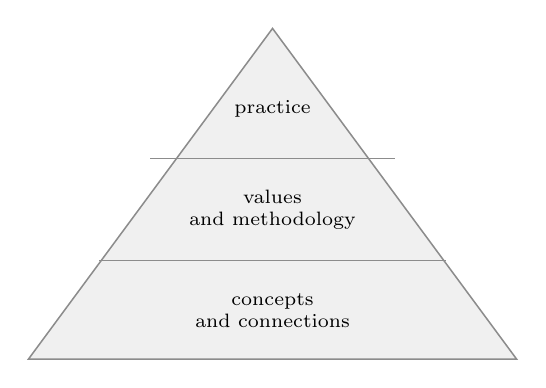
\begin{tikzpicture}[font=\scriptsize, line width=0.55pt]
  \coordinate (A) at (0,0);
  \coordinate (B) at (6.2,0);
  \coordinate (C) at (3.1,4.2);
  \draw[fill=gray!12, draw=black!45] (A) -- (B) -- (C) -- cycle;
  \draw[draw=black!45] (0.9,1.25) -- (5.3,1.25);
  \draw[draw=black!45] (1.55,2.55) -- (4.65,2.55);
  \node[align=center] at (3.1,0.62) {concepts\\and connections};
  \node[align=center] at (3.1,1.9) {values\\and methodology};
  \node[align=center] at (3.1,3.18) {practice};
\end{tikzpicture}
\end{adjustbox}
\end{center}

Concepts come first because a person cannot improve what they cannot name. ``Attention,'' ``capital,'' ``safety,'' ``future,'' and ``falling behind'' are not slogans. They are tools for seeing.

Values and methodology come next. Once you can see the problem, you still need standards and ways of deciding. What counts as progress? What counts as evidence? Which comparison is useful, and which comparison is merely emotional? What should be measured by rank, by ratio, by time, or by compounding?

Practice sits at the top because no concept becomes power until it enters action. Writing is an example. It is partly intellectual, but it is also physical. If you write continuously, you become better at writing. If you only admire writing, criticize writing, or plan to write, nothing much happens.

The same is true for learning, investing, selling, designing, teaching, programming, and building a personal business model. There is no mystery in the first step: do the work often enough that reality can correct you.

\section*{A Useful Definition}

So what does it mean to fall behind?

A practical definition is this:

\begin{quote}
You are falling behind when the standards of the world are rising faster than your ability, judgment, and capital can grow.
\end{quote}

This definition is better than comparing income, title, school, or surface lifestyle alone. It points to growth rate. A person with little money but a high learning rate may be moving forward. A person with a comfortable income but no new capacity may already be decaying.

Ask the question in a narrow field, not in life as a whole. Are you in the top 20\% of any useful ability among the people around you? If yes, what exactly is that ability, and how did you get there? If no, what ability could reasonably become your first leading edge?

Do not answer with determination alone. Determination is cheap when it has no schedule, no measurement, and no discomfort. A better answer has steps: what to study, what to practice, what to produce, whom to compare with, what feedback to accept, and how long to continue before judging.

\section*{Crisis Without Panic}

A sense of crisis can easily become anxiety. Anxiety consumes attention, and attention is the first form of wealth. So the goal is not to live in panic. The goal is to convert anxiety into directed practice.

The conversion looks like this:

\begin{center}
\begin{adjustbox}{max width=\linewidth}
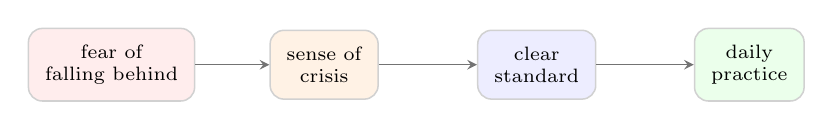
\begin{tikzpicture}[font=\scriptsize, line width=0.55pt, >=stealth]
  \node[draw=black!18, fill=red!7, rounded corners=5pt, align=center, inner sep=6pt] (fear) at (0,0) {fear of\\falling behind};
  \node[draw=black!18, fill=orange!10, rounded corners=5pt, align=center, inner sep=6pt] (crisis) at (2.7,0) {sense of\\crisis};
  \node[draw=black!18, fill=blue!7, rounded corners=5pt, align=center, inner sep=6pt] (standard) at (5.4,0) {clear\\standard};
  \node[draw=black!18, fill=green!8, rounded corners=5pt, align=center, inner sep=6pt] (practice) at (8.1,0) {daily\\practice};
  \draw[->, draw=black!55] (fear) -- (crisis);
  \draw[->, draw=black!55] (crisis) -- (standard);
  \draw[->, draw=black!55] (standard) -- (practice);
\end{tikzpicture}
\end{adjustbox}
\end{center}

The wrong response to crisis is self-comfort: at least I am better than someone. The right response is self-audit: where am I deceiving myself?

Spend thirty minutes a day for one week asking that question seriously. In which ability do you assume you are above average without evidence? Where are you protected by a small pond? Where do you use ``almost'' to avoid the hard part? Where do you say ``I could'' when the truth is only ``I have not''?

This is not an exercise in self-hatred. It is an exercise in positioning. A person who sees clearly can still move. A person who refuses to see clearly will be moved by others.

Raise your standards while the cost is still low. Many changes in this book begin as updated concepts. They require attention before they require money. That is both encouraging and frightening. Encouraging, because change is possible earlier than we thought. Frightening, because if the cost is low and we still refuse, the problem is no longer lack of opportunity.

To avoid falling behind, demand more from yourself. Not in every field, not in every hour, and not through theatrical exhaustion. Demand more in the specific places where the future is already asking for proof.

The future will not ask whether you felt average. It will ask what you can actually do.
